\section{Identifikationd der Reaktionsprodukte mithilfe von LC-MS}

Die Produkte der Reaktion mit Essigsäureanhydrid konnten ebenfalls mithilfe von \gls{lcms} identifiziert werden. In Abbildung 

\begin{figure}[!htbp]
  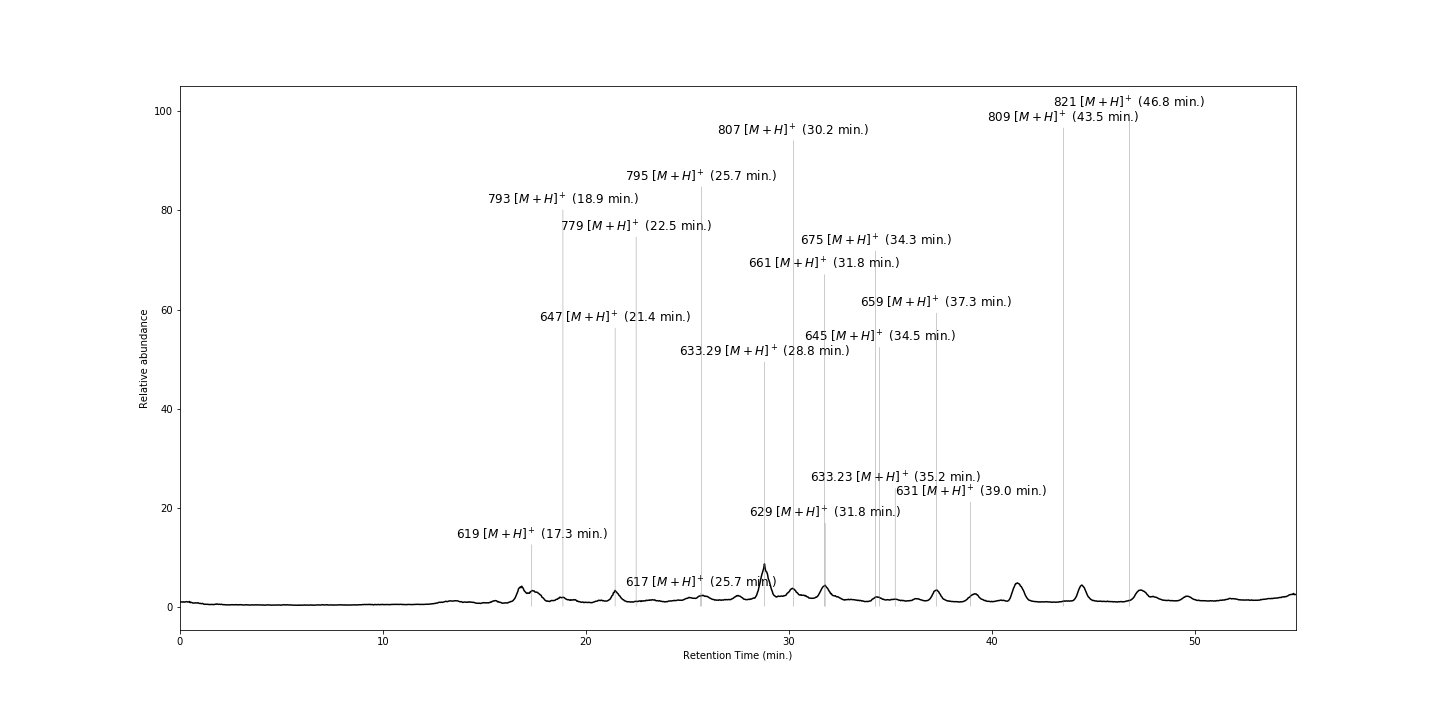
\includegraphics[width=\textwidth]{figures/Kapitel6/Reaktion3h/Kuerbis_Analyse_Reaktion3h_Ganzes_Spektrum.png}
  \caption[LC-MS Chromatogramm nach 3h Reaktionsdauer, Quelle: Author]{\gls{lcms} Chromatogramm}
  \label{fig:LCMSCChromatogrammRP}
\end{figure}


\begin{figure}[!htbp]
  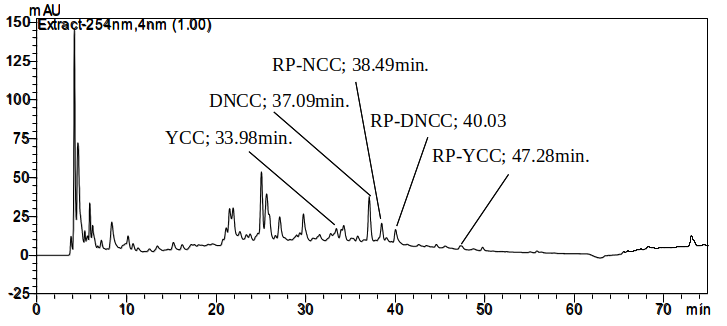
\includegraphics[width=\textwidth]{figures/Kapitel6/Reaktion3h/HPLC_Chromatogramm.png}
  \caption[HPLC Chromatogramm nach 3h Reaktionsdauer, Quelle: Author]{\gls{hplc} Chromatogramm}
  \label{fig:HPLCChromatogrammRP}
\end{figure}
